\section{Durchführung}
\label{sec:Durchführung}
Im Versuch stehen das in Abbildung \ref{fig:geraet} dargestellte Gerät und ein
Speicheroszilloskop zur Verfügung.

\begin{figure}
  \centering
  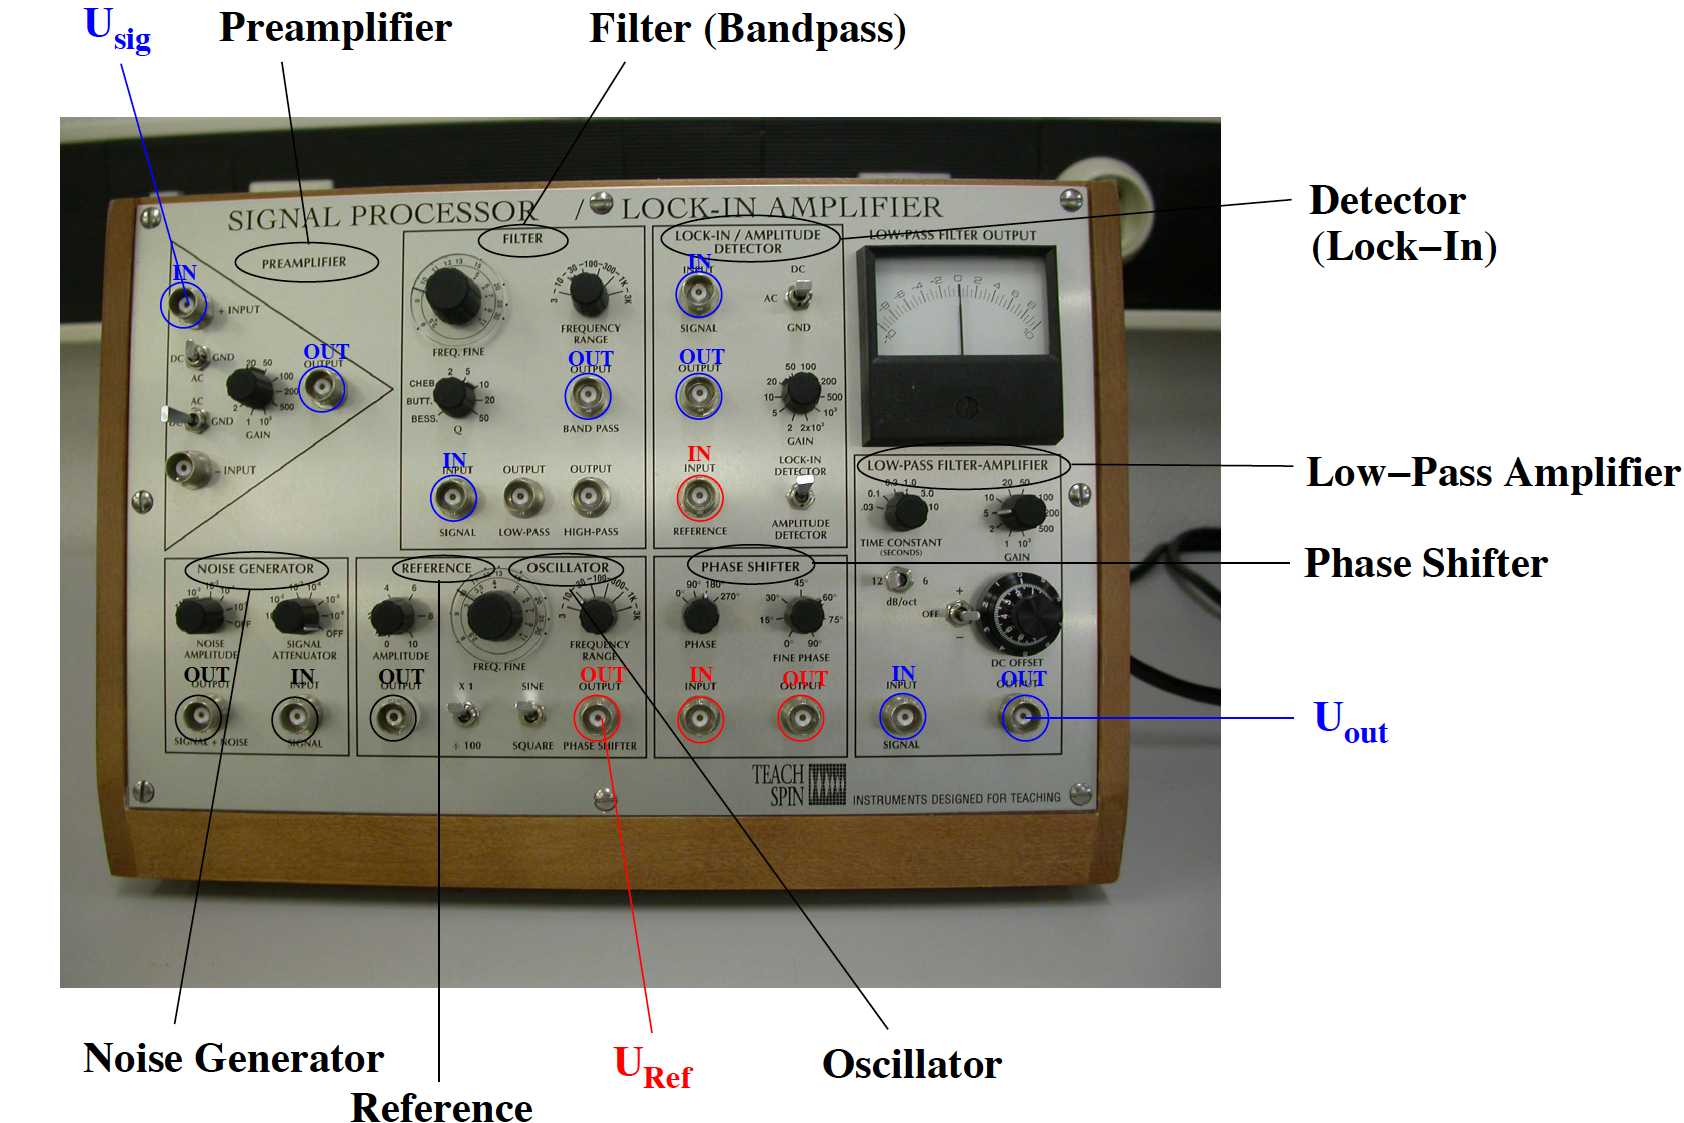
\includegraphics[width=\textwidth]{data/geraet.png}
  \caption{Darstellung des Gerätes mit Beschriftung der einzelnen Funktionen
  \cite{Versuchsanleitung}}
  \label{fig:geraet}
\end{figure}


Zunächst wird der Frequenzgenerator untersucht, indem beide verfügbaren
Ausgänge am Oszilloskop dargestellt werden. Anschließend werden möglichen Einstellungen
variiert und die Veränderungen des Signals auf dem Oszilloskop beobachtet. So soll
festgestellt werden, bei welchem der beiden Ausgänge die Amplitude der erzeugten
Spannung variabel und bei welchem sie fest ist und welchen Wert diese hat. Zudem
werden Bilder von jedem Ausgang bei je einer Einstellung gemacht.

Daraufhin wird die Schaltung aus \ref{fig:aufbau} aufgebaut, wobei der Noise Generator
auf OFF gestellt wird. Als Signalspannung wird im Frequenzgenerator eine sinusförmige Spannung
$U_{\symup{sig}}$ der Frequenz $f=1$\,kHz und der Amplitude $U_0=10$\,mV erzeugt.
Diese wird mit  einer ebenfalls sinusförmigen Referenzspannung $U_{\symup{ref}}$
derselben Frequenz multipliziert. Auf dem Oszilloskop wird die Ausgangsspannung
$U_{\symup{out}}$ ausgegeben. Für fünf verschiedene Phasen werden Bilder der
Ausgangsspannung gemacht. Zudem werden Messwerte für die integrierte Ausgangsspannung
in Abhängigkeit von der Phase aufgenommen.

\begin{figure}
  \centering
  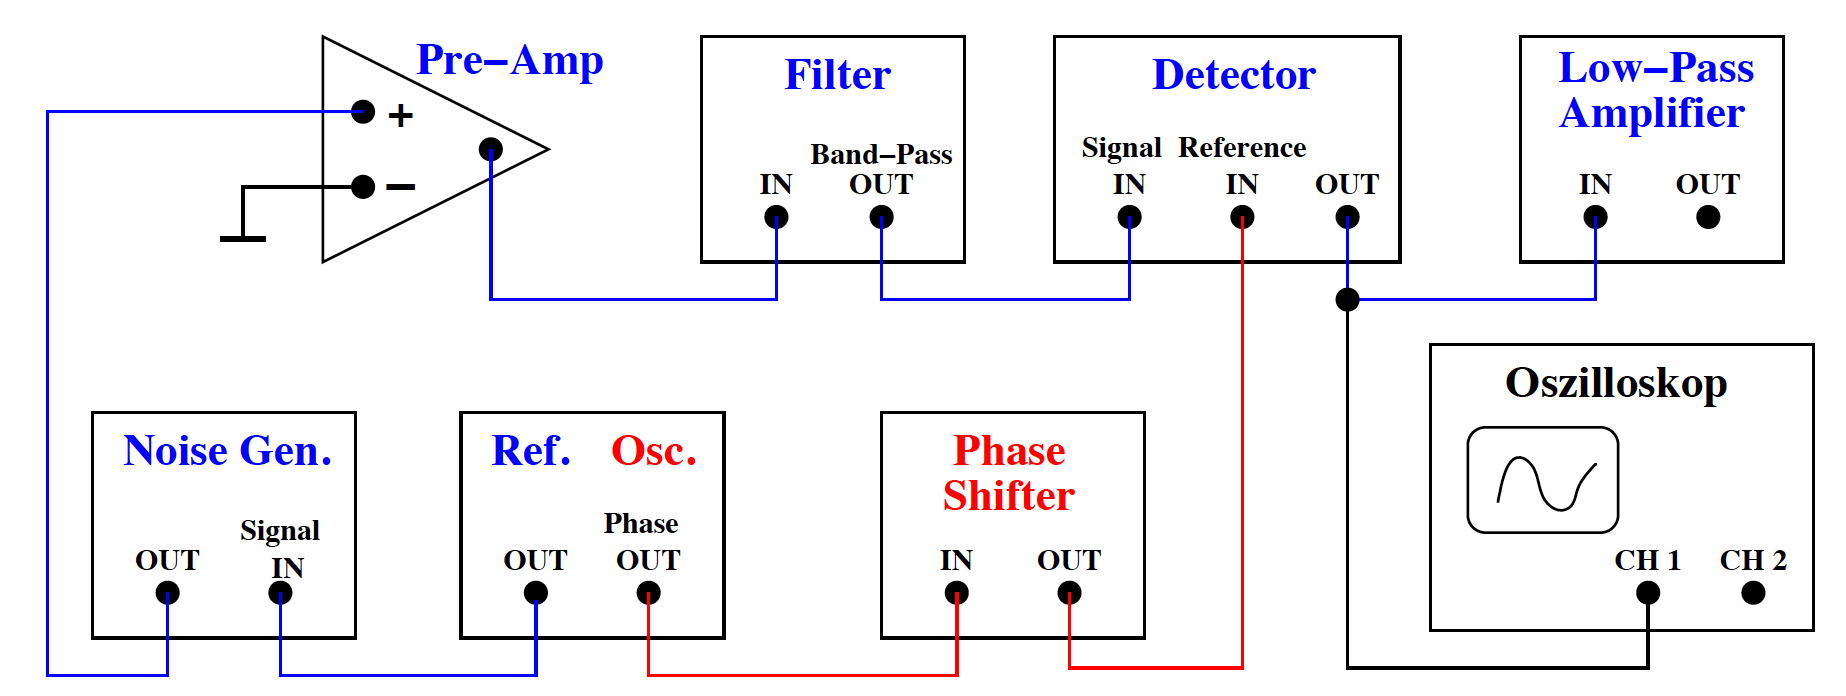
\includegraphics[width=\textwidth]{data/aufbau.png}
  \caption{Aufbau des im Versuch verwendeten Lock-In Verstärkers\cite{Versuchsanleitung}}
  \label{fig:aufbau}
\end{figure}

In der darauffolgenden Versuchsreihe wird nun der Noise Generator eingeschaltet.
Durch Darstellung des Ausgangs desselben auf dem Oszilloskop wird eine Einstellung für eine
Amplitude des Rauschens in der Größenordnung der Signalspannung gesucht. Ist diese
gefunden, so werden die oben beschriebenen Messungen erneut durchgeführt.
